\documentclass[conference]{IEEEtran}
%\documentclass[twocolumn,letterpaper,10pt]{article}
\usepackage{times}
\usepackage{graphicx,url}
\usepackage{listings}
\usepackage{subfigure}
\usepackage{multirow}
\usepackage{pictexwd}
\usepackage[absolute]{textpos}
\usepackage[english]{babel}
\usepackage{paralist}

\lstset{keywordstyle=\bfseries,
  flexiblecolumns=true,
  showstringspaces=false,
  breaklines=true
}
\lstloadlanguages{[ANSI]C++,HTML}
\lstdefinestyle{prg} {basicstyle=\tiny\sffamily, showspaces=false}


\newcommand{\prg}[3][ht!]{
\begin{figure}[#1]
  \lstinputlisting[language=C++,style=prg,showspaces=false,frame=single,breaklines=true,numbers=left,stepnumber=1,numbersep=-5pt]{fig/#2.cc}
  \caption{#3}
  \label{prg:#2}
\end{figure}
}

\newcommand{\fig}[4][ht!]{
	\begin{figure}[#1]
	{\centering{\includegraphics[#4]{fig/#2}}\par}
	\caption{#3}
	\label{fig:#2}
	\end{figure}
}

\def\sharedaffiliation{%
\end{tabular}
\begin{tabular}{cc}}

\begin{document}

\title{On the Influence of Shared Memory Contention in Real-time Multicore Applications}
	
\author{Blind Review}

%\author{Giovani Gracioli\IEEEauthorrefmark{1}, 
%Rafael Luiz Cancian\IEEEauthorrefmark{1}, 
%Wolfgang Schr\"{o}der-Preikschat\IEEEauthorrefmark{2}, 
%Ant\^{o}nio Augusto Fr\"{o}hlich\IEEEauthorrefmark{1}\\
%\\
%\begin{tabular}{cc}
%\IEEEauthorrefmark{1}Software/Hardware Integration Lab & \IEEEauthorrefmark{2}Department of Computer Science 4\\
%Federal University of Santa Catarina & Friedrich-Alexander University Erlangen-Nuremberg\\
%Florian\'{o}polis, Brazil & Erlangen, Germany\\
%\{giovani,cancian,guto\}@lisha.ufsc.br & wosch@informatik.uni-erlangen.de
%\end{tabular}
%}

\maketitle
\thispagestyle{empty}

\begin{abstract}
The continuous evolution of processor technology has allowed the utilization of multicore architectures in the embedded system domain. A major part of embedded systems, however, are inherently real-time (soft and hard) and the use of multicores in this domain is not straightforward due to their unpredictability in bounding worst-case execution scenarios. One of the main factors for unpredictability is the coherence through memory hierarchy. This paper characterizes the influence of contention for shared data memory in the context of embedded real-time applications. By using a benchmark, we have measured the impact of excessive shared memory invalidations on five processors with three different cache-coherence protocols (MESI, MOESI, and MESIF) and two memory organization (UMA and ccNUMA). Results have shown that the execution time of an application is affected by the contention for shared memory (up to 3.8 times slower). We also provide an analysis on Hardware Performance Counters (HPCs) and propose to use them in order to monitor and detect excessive memory invalidations at run-time.
\end{abstract}
   
%Shared memory contention, cache coherency, multicore processors.

\section{Introduction}

%DRAFT: Aplicações podem ser implementadas como ASICs. Exemplo
Several embedded real-time applications are implemented in a dedicated hardware logic (i.e., \textit{ASICs}) to obtain maximum performance and fulfill all the application's requirements (processing, real-time deadlines, etc). For instance, digital signal processing algorithms and baseband processing in wireless communication, should process a big amount of data under real-time conditions. Nevertheless, as they are usually implemented in a dedicated hardware, these applications present restrictions in terms of developing support (e.g., bug fixes, updating, and maintainability).

%DRAFT: SMP tem sido usados para RT. Aplicações executam sobre RTOS e são compostas de threas
The continuous evolution of processor technology, however, %together with its decreasingly cost, 
has enabled multicore (e.g. \textit{Symmetric Multiprocessing - SMP}) architectures to be also used in the embedded real-time system domain~\cite{Cho2006}. %Thus, the same applications can be ported to software, with similar performance and more support flexibility to their developers. 
In this context, an application is implemented on top of a Real-Time Operating System (RTOS), composed of several real-time cooperating threads (threads that share data). 

%DRAFT: Características do SMP devem ser consideradas, incluindo hierarq. mem., que afeta WCET
In this scenario, due to multicore processor organization, some important characteristics must be considered, specifically, the memory hierarchy~\cite{Muralidhara:2010, Zhuravlev:2010}. The memory hierarchy holds an important role, because it affects the estimation of the Worst-Case Execution Time (WCET), which is extremely important in the sense of guaranteeing that all threads will meet their deadlines through the design phase evaluation (schedulability analysis)~\cite{Marwedel2005, Suhendra2008, Wilhelm:2008}.

%DRAFT: 
Several works have been proposed to deal with memory organization in multicore architectures and provide real-time guarantees~\cite{Cho2006, Calandrino:2009, R:Davis:2009d}, but they only consider scenarios where threads are independent, that is, there is not data sharing. %In this case, the influence among threads (contention for cache space and interference in the cache lines) can be solved by some memory partitioning/locking mechanism provided by a special hardware~\cite{Suhendra2008} or implemented into the (real-time) scheduler~\cite{Guan2009, Zhuravlev:2010}. Partitioning/Locking techniques avoid overlapping of shared cache spaces and reduce the contention for the shared resource, increasing the application's throughput.
In situations where threads share data in a cooperating fashion, a partitioning/locking mechanism does not avoid the contention for shared data. For instance, consider a scenario composed of ``n" threads sharing data, running on ``m" different cores in a pipeline order (thread 2 after thread 1, thread 3 after thread 2, and so on). Thread 1 executes and writes in the shared data location. When the thread 2 accesses the shared data, it gets an invalid access and must ask (snoop request) for the most recent copy of the data or recover it from a lower memory level. The task of performing a snoop request is done automatically by the memory controller hardware, which increases the threads' execution time, even without their knowledge. The time to complete a snoop request is considerably slow (comparable to access the off-chip RAM)~\cite{BoydWickizer:10}, which can lead to an unexpected increase of the thread's execution time and deadline losses. 

%\fig{coop_threads}{An example of pipeline application composed of threads sharing data.}{width=.21\textwidth}

In this paper, we bring the problem of contention for shared memory to the embedded real-time system domain by measuring its influence on five different modern processors with three different cache-coherence protocols (MESI, MOESI, and MESIF)\footnote{Further information about cache-coherence protocols can be found in~\cite{Patterson:06,amd64,intel}.} and two memory organization (UMA and ccNUMA). We use a benchmark composed of two versions of the same application (sequential and parallel). If the sequential version is schedulable (proved by a schedulability analysis), the parallel version should be schedulable as well (it executes the same code but in parallel). We demonstrate in our experiments that due to the current multicore memory organization, the parallel version has its execution time affected (up to 3.8 times slower), which can lead to deadline losses. In order to monitor and detect when data sharing occurs, we also provide an analysis of Hardware Performance Counters (HPCs) in one multicore processor. HPCs are special registers available in the most modern microprocessors through the hardware Performance Monitoring Unit (PMU). They offer support to counting or sampling several micro-architectural events at run-time~\cite{Sprunt:02} and can be used to capture hardware events that reflect the software behavior. 

%Towards a solution, we envision an environment where the operating system (OS) real-time scheduler, together with a memory partitioning and Hardware Performance Counters (HPCs) support, could detect excessive memory invalidations among threads and take a decision (scheduling) in order to avoid deadline losses. Scheduling is a good solution because it does not require special hardware support and is easily integrated in practically any RTOS~\cite{Zhuravlev:2010}. Moreover, the scheduler is completely transparent to applications, that is, there is no need to change the application source code neither OS APIs nor libraries.

In summary, in this paper, we make the following contributions:

\begin{inparaenum}[(I)]
	\textbf{\item} We motivate the problem by measuring the influence of contention for shared memory in the context of hard real-time applications. % where deadlines must be always met.
	\textbf{\item} We evaluate the problem on five different multicore processors, with three different cache-coherence protocols (MESI, MOESI, and MESIF) and two memory organization (UMA and ccNUMA) by using a benchmark composed of a sequential and parallel versions of the same application.
	\textbf{\item} We evaluate HPCs in one of the five processors. HPCs together with the OS scheduler and memory partitioning are good alternatives to decrease the contention for shared data memory and provide predictability and performance gains to real-time applications. We present an analysis of hardware events that can be used to this purpose.
\end{inparaenum}

The remainder of this paper is organized as follows. %Section~\ref{sec:back} describes the problem and summarizes the background needed to follow the rest of the paper. 
Section~\ref{sec:benchmark} evaluates and discusses the problem. Section~\ref{sec:disc} analyzes some hardware events. Section~\ref{sec:related} provides an overview of related works, and Section~\ref{sec:conc} concludes the paper.

% \section{Problem Description and Background}
% \label{sec:back}
% 
% %\subsection{The Problem}
% 
% The problem we are addressing in this paper raises from the memory hierarchies present in the today's SMP architectures and their memory coherence protocols. When cores share data, each copy of the data is placed in the core's private cache and a cache-coherence protocol is responsible for keeping the consistency between each copy (through bus snooping).
% 
% \textbf{Problem}. When a core writes into a data that other cores have cached, the cache-coherence protocol invalidates all copies, causing an implicit delay in the application's execution time. At the same way, when a core reads a shared data that was just written by another core, the cache-coherence protocol does not return the data until it finds the cache that has the data, annotate that cache line to indicate that there is shared data, and recover the data to the reading core. These operations are performed automatically by the hardware and take hundreds of cycles (about the same time as accessing the off-chip RAM), increasing the application's execution time~\cite{BoydWickizer:10}. Two kinds of scaling problem occur due to shared memory contention~\cite{BoydWickizer:10}: access serialization to the same cache line done by the cache coherence protocol and saturation into the inter-core interconnection, preventing parallel processing gains. Reducing the effects of cache line contention can significantly improve the application's overall performance and avoid deadline misses. 
% 
% %The contention for shared memory causes an increase in the application's throughput and deadline losses. One can argue that there would be processing speedup by just turning the cache off and using the main memory directly. Nevertheless, it is a misconception that worst-case execution times with caches are equal to ones without caches~\cite{Liedtke:1997}. Moreover, it is common to find a considerable inter-thread interaction in multithreaded application. For example, some applications from NAS parallel and SPEC OMG benchmark suites have up to 20\% of inter-thread interaction, and up to 60\% of this interaction is affected by cache line contention~\cite{Muralidhara:2010}. 
% 
% %\subsection{Cache-coherence Protocols}
% 
% \textbf{Cache-coherence Protocols}. In general, there are three cache-coherence protocols being used in the today's multicore processors: MESI, MOESI, and MESIF. The MESI protocol is the most common cache-coherence protocol which supports write-back cache~\cite{Patterson:06}. A cache line in the MESI protocol can be marked as Modified (M - the cache line is present only in the current cache and its data is dirty), Exclusive (E - the cache line is present only in the current cache and it is clean), Shared (S - indicates that the cache line is shared by other caches and its state is clean), and Invalid (I - a cache line in this state does not hold a valid copy of data). The MOESI protocol adds a fifth state to the MESI protocol~\cite{amd64}. The Owned (O) state represents data that is both modified and shared. Therefore, there is no need to write modified data back to the memory before sharing it. The processor which holds a cache line in the O state is the only one to respond to a snoop request. The MESIF protocol includes a Forward (F) state that is used to respond to request for a copy of a cache line~\cite{intel}. MESI protocol is widely used in UMA architectures, such as Intel dual-core, while MESIF and MOESI are usually used in ccNUMA architectures, such as Intel Nehalem and AMD Opteron respectively.
% 
% %\subsection{Hardware Performance Counters}
% 
% \textbf{Hardware Performance Counters}. HPCs are special registers available in the most modern microprocessors through the hardware Performance Monitoring Unit (PMU). HPCs offer support to counting or sampling several micro-architectural events at run-time~\cite{Sprunt:02}. In multicore systems, for instance, it is possible to count the numbers of snoop requests, last-level cache misses, and evicted cache lines. In the next section we provide an analysis of the described problem by measuring the influence of shared memory contention through a benchmark. 

\section{Problem Evaluation and Discussion}
\label{sec:benchmark}

The problem we are addressing in this paper raises from the memory hierarchies present in the today's SMP architectures and their memory coherence protocols. %When cores share data, each copy of the data is placed in the core's private cache and a cache-coherence protocol is responsible for keeping the consistency between each copy (through bus snooping).
%\textbf{Problem}. 
When a core writes into a data that other cores have cached, the cache-coherence protocol invalidates all copies, causing an implicit delay in the application's execution time. At the same way, when a core reads a shared data that was just written by another core, the cache-coherence protocol does not return the data until it finds the cache that has the data, annotate that cache line to indicate that there is shared data, and recover the data to the reading core. These operations are performed automatically by the hardware and take hundreds of cycles (about the same time as accessing the off-chip RAM), increasing the application's execution time~\cite{BoydWickizer:10}. Two kinds of scaling problem occur due to shared memory contention~\cite{BoydWickizer:10}: access serialization to the same cache line done by the cache coherence protocol and saturation into the inter-core interconnection, preventing parallel processing gains. Reducing the effects of cache line contention can significantly improve the application's overall performance and avoid deadline misses

In order to evaluate the influence of contention for shared data memory in the execution time of an application, we have designed a benchmark to generate memory invalidatons composed of two versions of a pipeline application and a best-case application for comparing purposes (Figure~\ref{fig:apps}):

\begin{inparaenum}[(I)]
 \item \textbf{Sequential}: in this version, two functions are executed in a sequential order. There are no memory conflicts (Figure~\ref{fig:sequential}). The objective of this version is to simulate an algorithm % implemented in hardware, that is, the algorithm 
 that does not have shared memory invalidations.

 \item \textbf{Parallel}: two threads run at the same time and share data (Figure~\ref{fig:parallel}). The objective of this version is to evaluate the performance of the previous version when it is implemented in a multicore architecture. Both functions (1 and 2) from sequential and parallel versions have the same operations and memory accesses (see Figure~\ref{prg:app_loop}). Common sense dictates that this version should run about two times faster than the sequential one. Consequently, if the sequential version is schedulable (proved by a schedulability analysis), the parallel version should be schedulable as well. We do not use any kind of synchronization (i.e., semaphores, mutexes, or condition variables) to ensure the data consistency because we are only interested in measuring the shared data contention overhead.

 \item \textbf{Best-case application}: two threads run at the same time, but do not share data (Figure~\ref{fig:best-case}). This application should run about 2 times faster than the sequential one in a multicore processor. The objective is to have a best-case scenario comparable to the sequential and parallel versions.
\end{inparaenum}

\begin{figure}
\centering
\begin{tabular}{ccc}
	\subfigure[] {
	\fbox{
	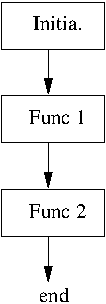
\includegraphics[scale=.5]{fig/seq_app}
 	\label{fig:sequential}}} 
	\subfigure[] {
	\fbox{
	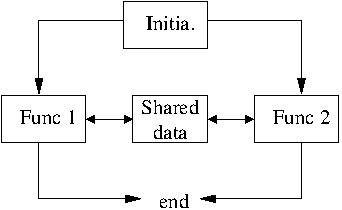
\includegraphics[scale=.5]{fig/par_app}
	\label{fig:parallel}}}
	\subfigure[] {
	\fbox{
	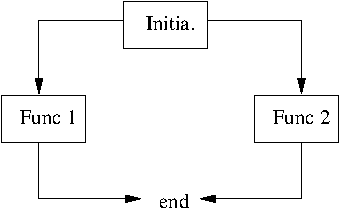
\includegraphics[scale=.5]{fig/best_case_app}
	\label{fig:best-case}}}\\
\end{tabular}
\caption{Benchmark applications: (a) sequential (b) parallel (c) best-case.}
\label{fig:apps}
\end{figure}

All three applications have two two-dimensional arrays of varying size ROWS x COLS and a loop of 10000 iterations, in which math operations are executed. The shared data in the parallel version is accessed by reading and writing in both arrays and in the same positions, thus we are sure that both threads are accessing the corresponding cache line. Figure~\ref{prg:app_loop} shows part of the source code from one of the functions implemented in the sequential and parallel versions. At initialization phase, the arrays are started with zero and the threads are created (parallel and best-case applications). The benchmark was implemented as a Linux application, in C++ (GNU g++ compiler), and using the pthread library version 2.11.12 for the parallel and best-case versions. Each thread in these versions was assigned to a different core by using the \emph{pthread\_setaffinity\_np} function. We ran each application version 10 times and then we extracted the sampled worst-case execution time. The time was measured by the Linux \emph{time} tool. The kernel version used in all test was the 2.6.32.
The arrays' size was set to 64x64 (32~KB), 128x128 (128~KB), 256x256 (512~KB), 512x512 (2~MB), 1024x1024 (8~MB), and 2048x2048 (32~MB), considering an integer as 4 bytes. 
Table~\ref{tab:processors} shows the  configuration of 3 processors used during the evaluations.

\prg{app_loop}{Part of the source code of sequential and parallel applications.}

\begin{table}
\begin{center}
\caption{AMD Opteron 280, Intel i5-650, and Intel Q9550 configurations.} %, Intel Xeon 5030, and PowerPC-based on Cell processors configurations.}
\footnotesize{
\begin{tabular}{|c|c|c|c|}%c|c|}
\hline
\textbf{Feature/} & \textbf{Opteron 280} & \textbf{Intel i5-650} & \textbf{Intel Q9550} \\%& \textbf{Xeon 5030} & \textbf{PowerPC} \\
\textbf{Processor}& & & \\
\hline
Frequency & 2.4 GHz & 3.2 GHz &  2.83 GHz \\%& 2.66 Ghz & 3.2 Ghz\\
\hline
%Instruction set & 64 bits & 64 bits & 64 bits & 64 bits & 64 bits \\
%\hline
Physical dies & 2 & 1 & 1 \\%& 2 & 1\\
\hline
Cores per die & 2 & 2 & 4 \\%& 2 & 2\\
\hline
SMT & - & 2 & - \\%& 2 & -\\
\hline
Bus Speed & HyperTransport  & QPI 1.3 GHz & FSB 1.3 GHz \\%& FSB 667 Mhz & 1.6 Ghz\\
	  & 1.0 GHz	    &  & \\
\hline
L1 private data& 128 KB 2-way& 32 KB &  64 KB \\%& 16 KB & 32 KB \\
cache size 		& associative  & 	   & 		\\%&	    &		\\  				
\hline
L2 cache & 1 MB 16-way  & 256 KB per   &  12 MB \\%& 4 MB 8-way  & 512 KB\\ 
size 	  & associative  & core (private)  &  		\\%& associative & 	  \\
\hline
L3 shared & - & 4 MB & - \\%& - & - \\
\hline
%Cache alignment & 64 bytes & 64 bytes & 64 bytes & 128 bytes & 64 bytes \\
%\hline
Memory 		& ccNUMA   & ccNUMA	  & UMA \\%& UMA & UMA\\
architecture 	&		   & 		  & 	\\%&	  &	   \\
\hline
Coherence & MOESI & MESIF & MESI \\%& MESI & MESI \\
protocol  &		  &		  &		 \\%&		&	   \\
%\hline
%Linux version & 2.6.32 & 2.6.32 & 2.6.32 & 2.6.32 & 2.6.32 \\
\hline
\end{tabular}
}
\end{center} 
\label{tab:processors}	
\end{table}

Figure~\ref{fig:q9550_eval} presents the WCET (in logarithm scale) for each application version on the Intel Core 2 Quad Q9550 processor. As expected, the best-case application was about 2 times faster than the sequential one. However, we note that, independently of the arrays' size, the parallel version was always slower than the sequential version (up to 1.31 time). The relative standard deviation for the sequential, parallel, and best-case applications was 0.78\%, 0.71\%, and 0.36\% of the total execution time, respectively. 
% Talvez o experimento abaixo possa ser retirado para caber em 8 páginas
In addition, we repeated the evaluation using an optimized version of the Linux kernel~\cite{BoydWickizer:10}. Basically, the Linux was modified to avoid locks and atomic instructions by reengineering data structures and unnecessary sharing. All applications presented similar performance, and the parallel version was always slower than the sequential one. This performance degradation is caused especially by data sharing (lines 9, 10, 13, and 14 of Figure~\ref{prg:app_loop}), which causes excessive invalidations in the same cache line due to the MESI cache-coherence protocol and bus snooping. Moreover, considering the embedded real-time domain, this performance degradation implies in deadline losses. %Figure~\ref{fig:q9550_opt} shows the measured WCET. All applications presented similar performance, and the parallel version was always slower than the sequential one. The relative standard deviation for the sequential, parallel, and best-case applications was 0.18\%, 1.73\%, and 0.29\%. For the application developer there is nothing wrong, since the problem comes from the current multicore processor architectures and not from the applications. 

\begin{figure}[ht!]
\centering
  \subfigure[] {
    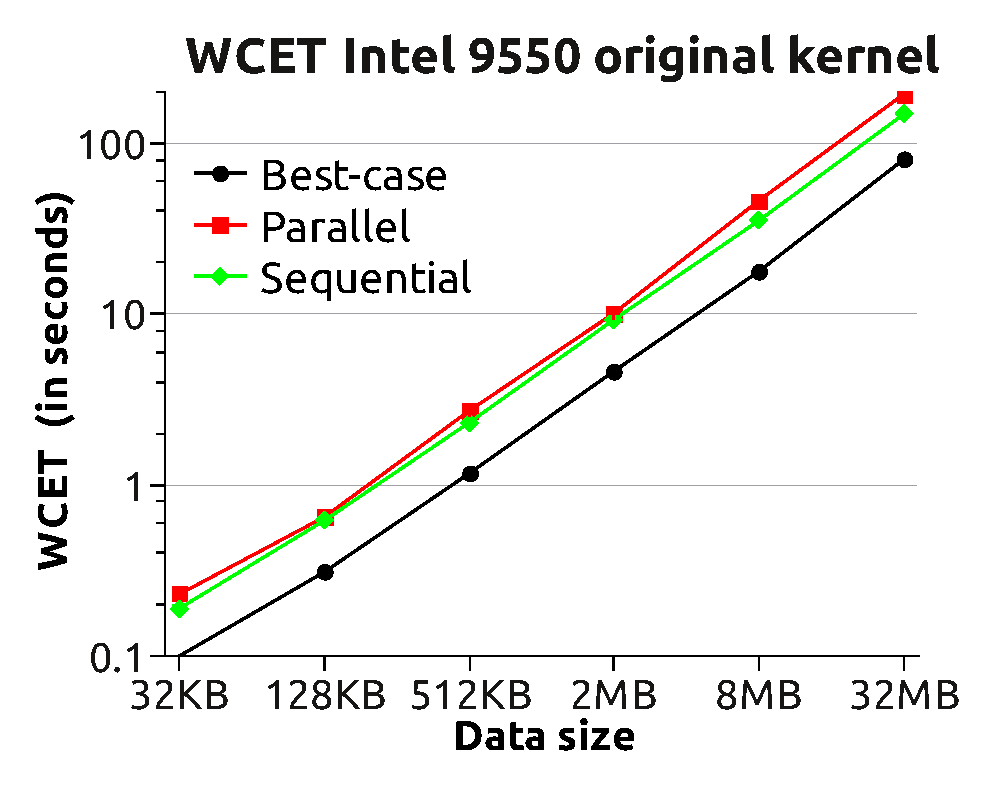
\includegraphics[width=.22\textwidth,height=3.25cm]{fig/q9550_original2}
    \label{fig:q9550_orig}
  }
  \subfigure[] {
    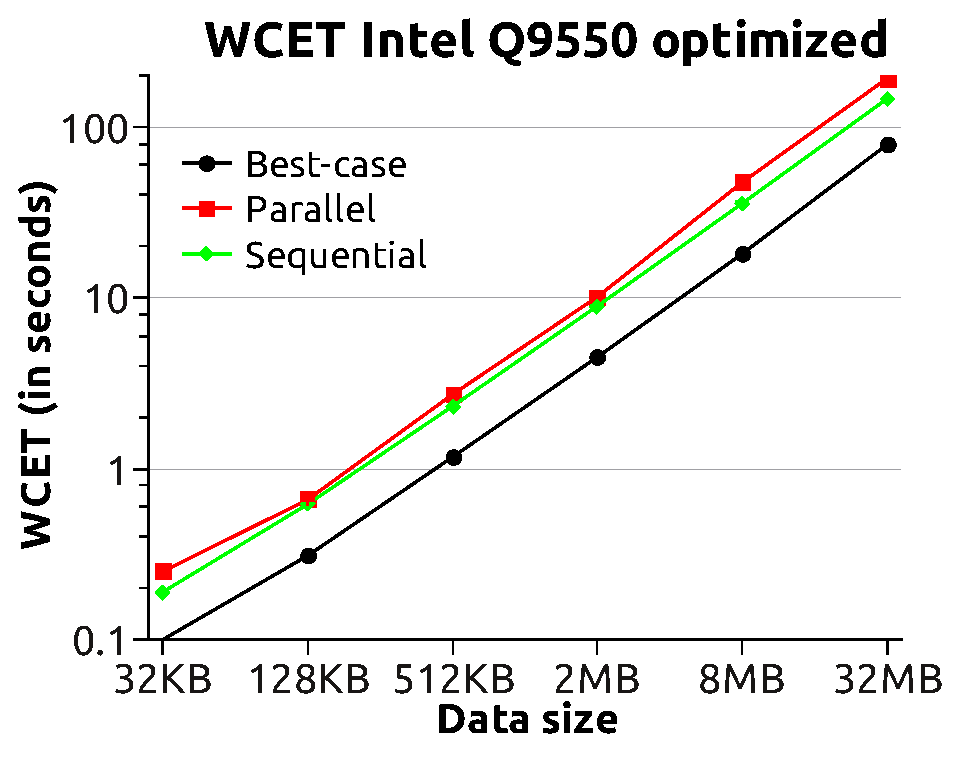
\includegraphics[width=.22\textwidth,height=3.25cm]{fig/q9550_optimized2}
    \label{fig:q9550_opt}
  }
\caption{Benchmark evaluation on Intel dual-core Q9550 processor: (a) Original Linux kernel (b) Optimized Linux kernel.}
\label{fig:q9550_eval}
\end{figure}
%tirar até aqui

We also ran the three applications in other two SMP processor, Intel Xeon 5030 and a PowerPC-based dual-core on the Cell architecture (MESI/UMA)\footnote{For reviewers: Due to space constraints, we suppress the graphs of these experiments.}. We obtained even worse execution times, for the PowerPC processor the parallel version was up to 2.62 times slower than the sequential one, while for the Intel Xeon 5030 the parallel was up to 3.87 times slower when the data size is 32~MB. For the Intel Xeon processor, the performance degradation increased due to bus saturation (FSB) caused by a greater frequency of data transfer between the L2 cache and the main memory and also by the cache-coherence protocol that writes the data back to memory.
%Both use MESI as cache-coherence protocol and are UMA architectures. 
%As the previous experiment, each thread in the parallel and best-case applications was assigned to a different core by using the \emph{pthread\_setaffinity\_np} function. Figure~\ref{fig:xeon_ppc_eval} shows the benchmark performance on the two processors. We obtained even worse execution times, for the PowerPC processor the parallel version was up to 2.62 times slower than the sequential one, when the data size is exactly the same size of the L2 cache (512~KB), while for the Intel Xeon 5030 the parallel was up to 3.87 times slower when the data size is 32~MB. The relative standard deviation for the sequential, parallel, and best-case applications in the PowerPC-based processor was 0.58\%, 1.39\%, and 0.68\% of the total execution time, and in the Intel Xeon 5030 processors it was 4.20\%, 1.07\%, and 4.38\%, respectively. We also assigned threads to different cores in relation with their physical location (threads in the same physical die and threads in different physical dies\footnote{By using the \emph{proc filesystem} (/proc/cpuinfo) is possible to gather this information.}) and observed that there is almost no variation in the WCET for these SMP/UMA processors. For the Intel Xeon processors, there is a linear increasing the execution time from 8~MB to 32~MB due to bus saturation (FSB) caused by a greater frequency of data transfer between the L2 cache and the main memory and also by the cache-coherence protocol that writes the data back to memory (write-back). The same phenomenon was not observed in the previous processor, where the L1 cache size is 4 times greater, the L2 cache size is 3 times greater, and the FSB is twice faster.

% \begin{figure}[ht!]
% \centering
% \subfigure[] {
% 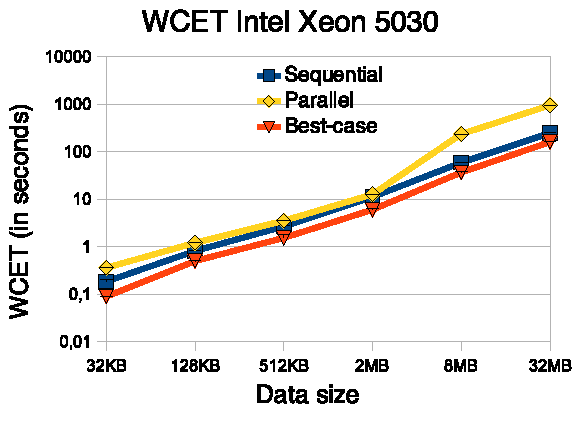
\includegraphics[width=.21\textwidth,height=3.25cm]{fig/xeon_5030}
% \label{fig:xeon_5030}
% }
% \subfigure[] {
% 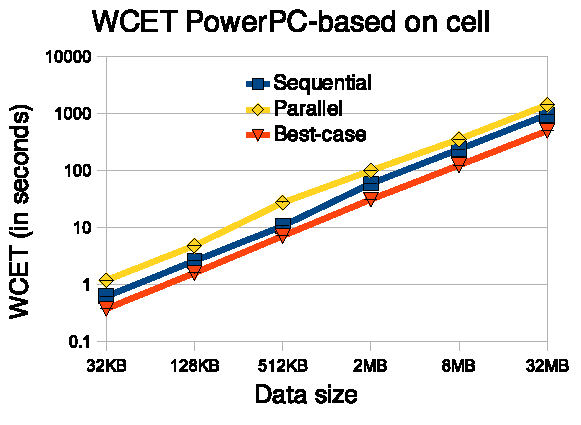
\includegraphics[width=.21\textwidth,height=3.25cm]{fig/powerpc_cpus_0_and_1}
% \label{fig:ppc_0_and_1}
% }
% \caption{Benchmark evaluation on (a) Intel Xeon 5030 and (b) PowerPC-based processors.}
% \label{fig:xeon_ppc_eval}
% \end{figure}

Our next evaluation was carried out in the AMD Opteron 280 processor (MOESI/ccNUMA - see Table~\ref{tab:processors}). %This processor implements MOESI as cache-coherence protocol and differ from the previous processors because it is a ccNUMA architecture. 
We evaluated two execution scenarios:

\begin{inparaenum}[(I)]
	%\item \textbf{Scenario 1}: threads running in cores in different dies (CPUS 0 and 1).
	\item \textbf{Scenario 1}: threads running in cores in the same die (CPUS 0 and 2).
	\item \textbf{Scenario 2}: Linux Completely Fair Scheduler (CFS) responsible for allocating a thread to a core. CFS supports the creation of groups of tasks, round-robin, FIFO, and real-time scheduling policies. Jones presents a complete description about the CFS implementation~\cite{Jones:2009}.
\end{inparaenum}

The objective of this experiment was to analyze the relation between the physical core location and the shared memory coherence by measuring the applications WCET. %Figure~\ref{fig:opt_0_and_1} shows the WCET for scenario 1. For data size of 8~MB and 32~MB the sequential application was slightly faster than the parallel one. For all other sizes, the parallel one was slower than the sequential. The relative standard deviation for the sequential, parallel, and best-case applications was 5.47\%, 5.34\%, and 6.57\% of the total execution time. 
Figure~\ref{fig:opt_0_and_2} shows the measured WCET for scenario 1. The parallel version was always slower than the sequential one (up to 2.82 times using arrays' size of 32~KB). We can also note a decreasing in the WCET difference as the arrays' size increases. The relative standard deviation in this scenario for the sequential, parallel, and best-case was 2.86\%, 9.88\%, and 4.29\%. Figure~\ref{fig:opt_cfs_linux} represents the measured WCET for scenario 2. The applications performance was similar to the scenario 1. The relative standard deviation for the sequential, parallel, and best-case was 4.68\%, 3.91\%, and 4.99\%. We also ran the threads in cores located in different dies, and the sequential application was slightly faster than the parallel one for data size of 8 and 32~MB. We can conclude that the WCET is related to the arrays' size, the bigger arrays' size the faster the execution time. Additionally, as expected from a ccNUMA processor, there is a variation in the WCET when executing applications in cores physically located in different dies.

\begin{figure}[htb]
\centering
%\subfigure[] {
%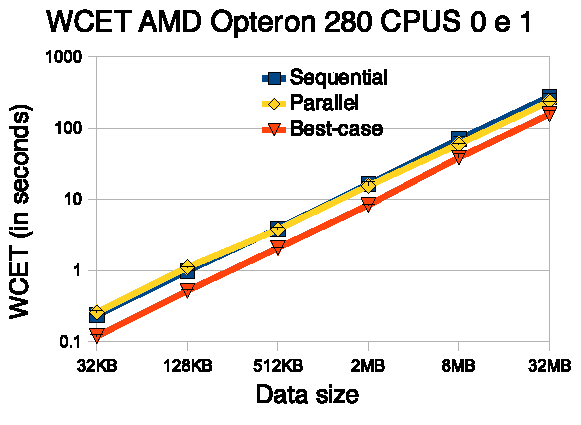
\includegraphics[width=.21\textwidth,height=3.25cm]{fig/opteron_cpus_0_and_1}
%\label{fig:opt_0_and_1}
%}
\subfigure[] {
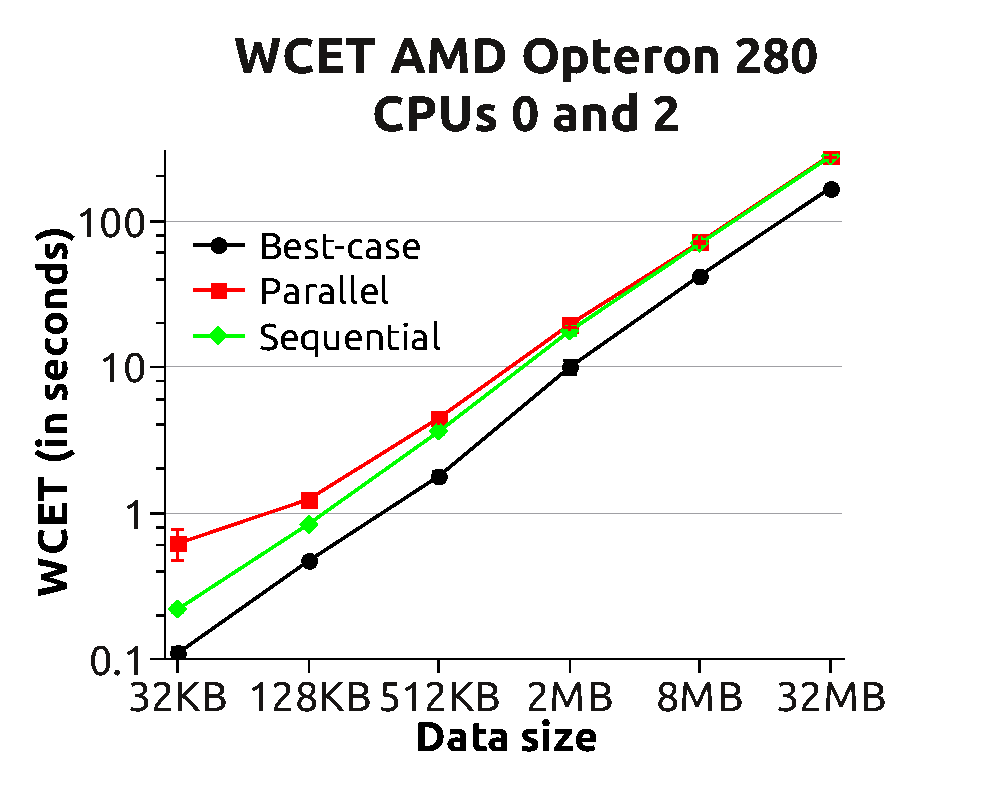
\includegraphics[width=.22\textwidth,height=3.25cm]{fig/opteron_cpus_0_and_22}
\label{fig:opt_0_and_2}
}
\subfigure[] {
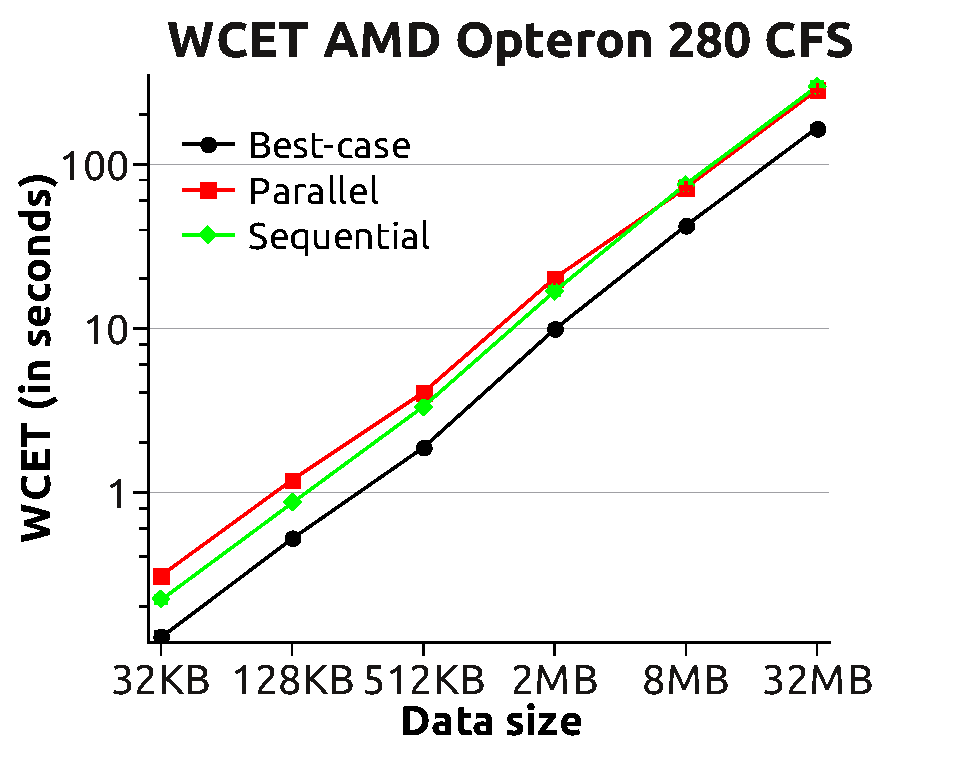
\includegraphics[width=.22\textwidth,height=3.25cm]{fig/opteron_cpus_random2}
\label{fig:opt_cfs_linux}
}
%\caption{Benchmark evaluation on AMD Opteron 280 processor assigning threads to specific cores: (a) CPUS 0 and 1 (b) CPUS 0 and 2 (c) Linux CFS scheduler.}
\caption{Benchmark evaluation on AMD Opteron 280 processor assigning threads to specific cores: (a) CPUS 0 and 2 (b) Linux CFS scheduler.}
\label{fig:opteron_eval}
\end{figure}

Our next evaluation was carried out in the Intel i5-650 processor (MESIF/ccNUMA - see Table~\ref{tab:processors}). We ran each application in two different scenarios:

\begin{inparaenum}[(I)]
	\item \textbf{Scenario 1}: threads running in two different cores (CPUS 0 and 1).
	%\item \textbf{Scenario 2}: threads running in the same core using \textit{Symmetric Multithreading} (SMT) technology (CPUS 0 and 2).
	\item \textbf{Scenario 2}: Linux CFS responsible for allocating a thread to a core.
\end{inparaenum}

Figure~\ref{fig:i5_eval} shows the WCET of each application in the two described scenarios. We can observe that the difference between the parallel and best-case WCET was almost the same in the two scenarios.  In general, the parallel version was faster than the sequential one and only in scenario 1 with data size of 32~MB it was slower than the sequential. The relative standard deviation of sequential, parallel, and best-case applications in scenario 1 was 0.95\%, 3.30\%, and 1.53\%, and in scenario 2 was 1.35\%, 3.07\%, and 2.92\% of the total execution time. The performance increasing can be explained by the processor organization, composed of Intel's QuickPath Interconnect (QPI) and MESIF protocol. Compared to the FSB, QPI provides higher bandwidth and lower latency for NUMA-based architectures. Each processor has an integrated memory controller and features a point-to-point link (all processors are connected), allowing parallel data transfer and shortest snoop request completion~\cite{intel}. 

%In scenario 2, the SMT obviously degrades performance of the parallel and best-case applications.

\begin{figure}[htb]
\centering
\subfigure[] {
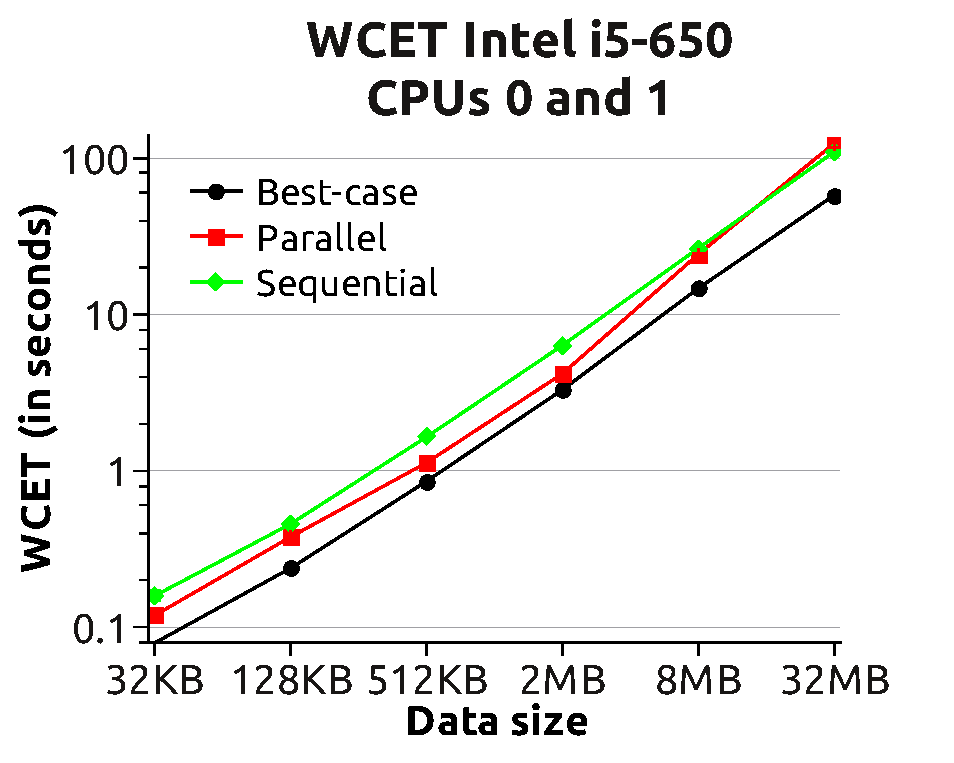
\includegraphics[width=.21\textwidth,height=3.25cm]{fig/intel-i5_cpus_0_and_12}
\label{fig:i5_0_and_1}
}
%\subfigure[] {
%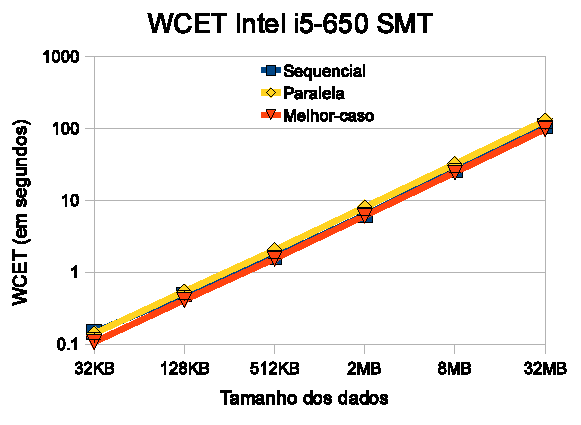
\includegraphics[width=.21\textwidth,height=3.25cm]{fig/intel-i5_cpus_0_and_2}
%\label{fig:i5_0_and_2}
%}
\subfigure[] {
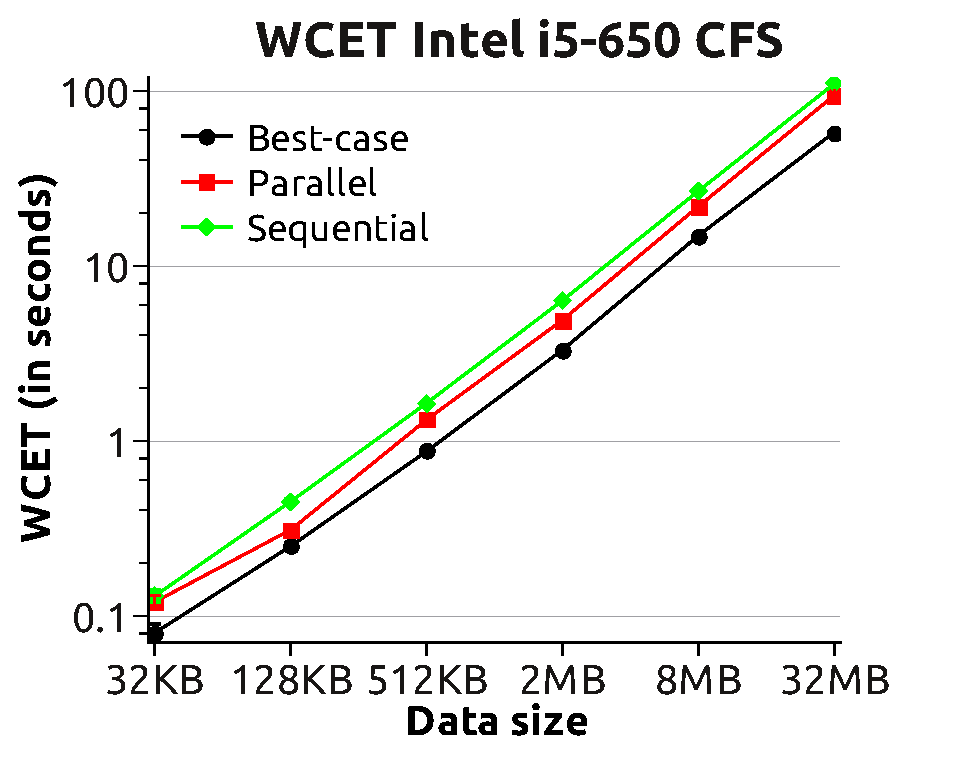
\includegraphics[width=.21\textwidth,height=3.25cm]{fig/intel-i5_cpus_random2}
\label{fig:i5_cfs_linux}
}
\caption{Benchmark evaluation on Intel i5-650 processor assigning threads to specific cores: (a) CPUS 0 and 1 (b) Linux CFS scheduler.}
\label{fig:i5_eval}
\end{figure}

\textbf{Discussion}. During our evaluations we observed a set of interesting facts regarding the evaluated problem:

\textbf{SMP architectures:} We executed our benchmark on five different processors that implement MESI, MESIF, and MOESI, as cache-coherence protocol, and two different memory organizations (ccNUMA and UMA). The five processors have proved that the impact of memory coherence is not negligible and should be mainly considered for real-time and processing intensive applications. The ccNUMA processors have suffered less impact considering the contention for shared data due to their bus, cache-coherence protocol, and memory organizations. However, because its different memory access times and unpredictability, ccNUMA architectures are not the most adequate for real-time applications. A execution time degradation up to 3.8 times for the parallel application compared to the sequential one was obtained using the Intel Xeon 5030 processor, which can certainly violate real-time guarantees if not correctly handled.
%%%%%%%%%%%%%%%%%%%%%%%%%%%%%%%%

\textbf{Memory partitioning:} In order to reduce cache line invalidations and the interference among threads that do not share resources, methods such as memory partitioning~\cite{Muralidhara:2010} could be used. However, in a cooperating real-time application, such as those found in digital signal processing area, where threads share data, memory partitioning does not solve the problem because threads will access the same data location on the memory hierarchy. Memory partitioning can be used together with other techniques, such as scheduling, in order to decrease the contention for shared resources between several applications and application's threads.

\textbf{Operating systems:} We used the Linux operating system. In general, OSs do not have any support for handling the contention for shared data. Moreover, the state-of-art real-time multicore scheduling algorithms do not consider the problem. Scheduling is a good alternative to solve the problem because it is totally transparent to applications, there is no need to change APIs nor libraries, and can be easily integrated in RTOS. HPCs can be used to provide to the OS scheduler information about data sharing. The next section provides an analysis of some hardware events that can be used to this purpose.

\section{HPCs Analysis}
\label{sec:disc}

HPCs are a good alternative to monitor shared memory invalidations and provide to the OS a correct view of the application behavior. The current related works neither %do not 
take into consideration the problem nor provide an analysis of available HPCs. Hence, our objective is to analyze the main hardware events that could be used to monitor shared memory invalidations at run-time. Observing the events available in the Intel Core 2 Q9550 processor, we identified that the following events are interesting to our purpose because they provide information about cache lines and bus snooping~\cite{intelsys}:

\begin{inparaenum}[(I)]
	%\item Last-level cache misses: counts the number of misses in the last-level cache. 
	\item \textbf{L2 cache requests:} counts all completed L2 cache requests. This event can count occurrences of accesses to cache lines at different MESI states. Since data sharing and invalidations are generated when lines are in S or I states, we monitor all L2 cache requests for these two states.
	\item \textbf{L1 data cache snooped by other core:} counts the number of times the L1 data cache is snooped for a cache line that is needed by the other core in the same processor. The cache line is either missing in the data cache of the other core or is available for reading only and the other core wishes to write the cache line. We monitor all snoops for cache lines in S and I states.
	\item \textbf{External snoops:} counts the snoop responses to bus transactions. We monitor all snoop responses to bus transactions that found a cache line in the modified state (HITM).
\end{inparaenum}

%\fig{HPC_llc_misses}{Number of last-level cache misses.}{width=.21\textwidth}

We use the \emph{perf} Linux tool to read the HPCs and the \emph{libpfm4} to list all available HPCs and use them as input to \emph{perf}. We ran each application 
(Figure~\ref{fig:apps}) and each event configuration for 10 times and extracted the average value. All tests were executed in the Intel Q9550 processor using Linux 2.6.32. 

Figure~\ref{fig:HPC_rqsts} shows the measured values for the L2 cache request events (in logarithm scale). In Figure~\ref{fig:hpc_l2_i}, we can note an exponential increase in the events for the sequential and best-case application after 2~MB. When the data size is 32~MB, all the three application have similar behavior because the data size is greater than the L2 cache size. Consequently, there is more data being replaced from/to the cache to/from the main memory and thus more invalid cache lines. Hence, this event is not a good alternative to monitor shared memory invalidation for data sizes greater than 2~MB.

\begin{figure}[ht!]
\centering
	\subfigure[] {
	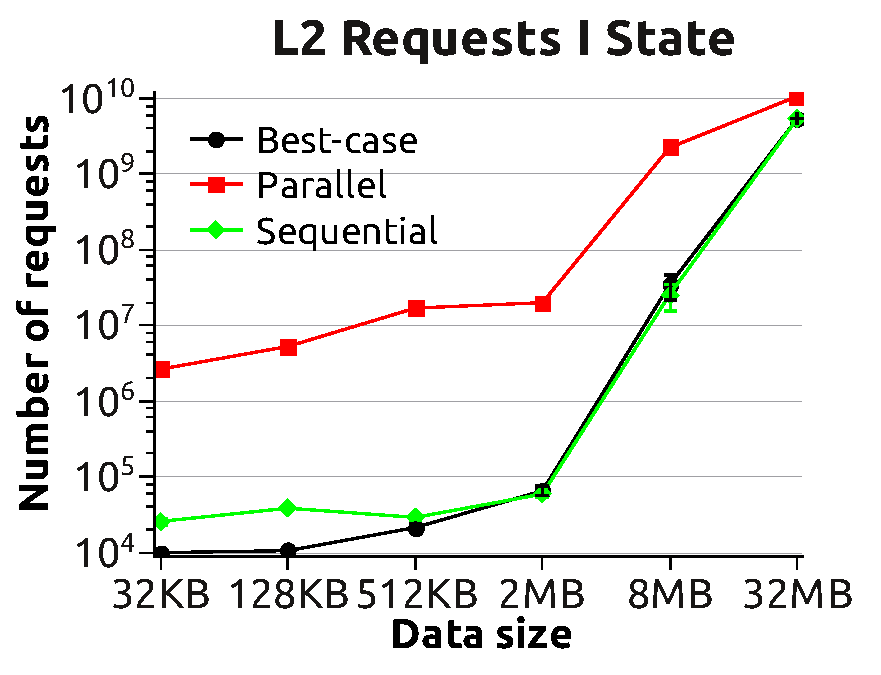
\includegraphics[width=.22\textwidth,height=3.25cm]{fig/HPC_l2_rqs_I_state2}
	\label{fig:hpc_l2_i}
	}
	\subfigure[] {
	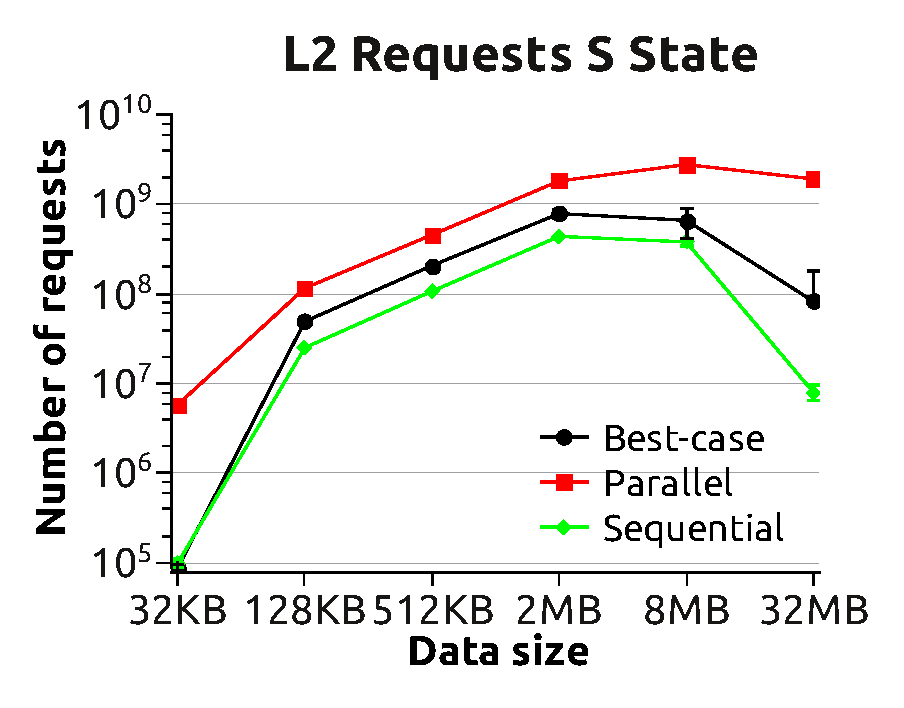
\includegraphics[width=.22\textwidth,height=3.25cm]{fig/HPC_l2_rqs_S_state2}
	\label{fig:hpc_l2_s}
	}
\caption{Benchmark HPCs evaluation on Intel Q9550 processor: L2 requests for (a)  I state and (b) S state.}
\label{fig:HPC_rqsts}
\end{figure}

Figure~\ref{fig:hpc_l2_s} shows the L2 cache requests for lines in the shared state. The difference among the three applications was not too significant. The explanation for shared data in the sequential and parallel applications is the natural implementation of a multicore kernel, where mutual exclusion of shared data structures is guaranteed by shared spin locks. When the data size is greater than the half size of the L2 cache, we observe a reduction in the cache lines in S state and an increasing of cache lines in I state. As both threads in the parallel version are always writing into the shared data, this event has shown not to be a good alternative to measure memory invalidations.

The next evaluation measured the number of times the L1 data cache is snooped by another core. Figure~\ref{fig:snoop_req} shows the obtained values of snoops for cache lines in I state (Figure~\ref{fig:snoops_i}) and S state (Figure~\ref{fig:snoops_s}). There is a greater difference in the number of snoops between the parallel and the other two applications considering snoops for cache lines in I state, as also observed in Figure~\ref{fig:HPC_rqsts}. The parallel version has obtained up to 2 order of magnitude more snoops than the sequential and best-case applications. As the data size increase, there is more false sharing occurring, more data being replaced in the cache, and consequently more snoops. False sharing occurs when threads running on different cores access data addresses that are in the same cache line. As conclusion for this event, the number of snoops for cache lines in I state is a good option for monitoring shared data invalidations.

\begin{figure}[ht!]
\centering
	\subfigure[] {
	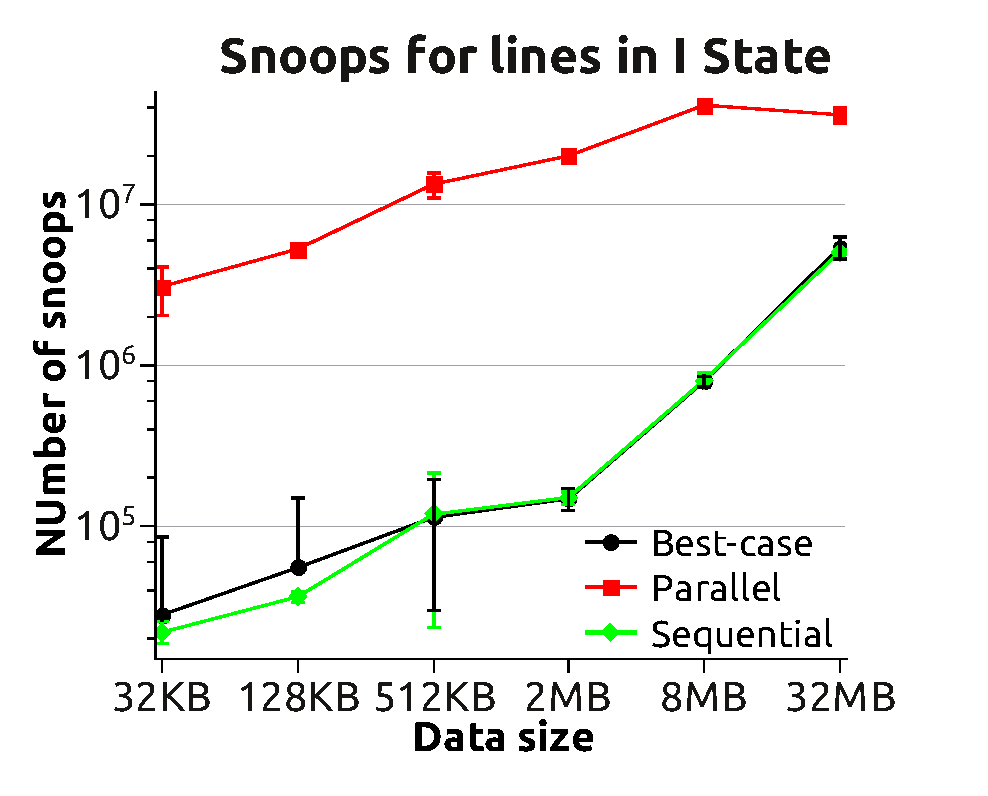
\includegraphics[width=.22\textwidth,height=3.25cm]{fig/HPC_snoop_invalidate2}
	\label{fig:snoops_i}
	}
	\subfigure[] {
	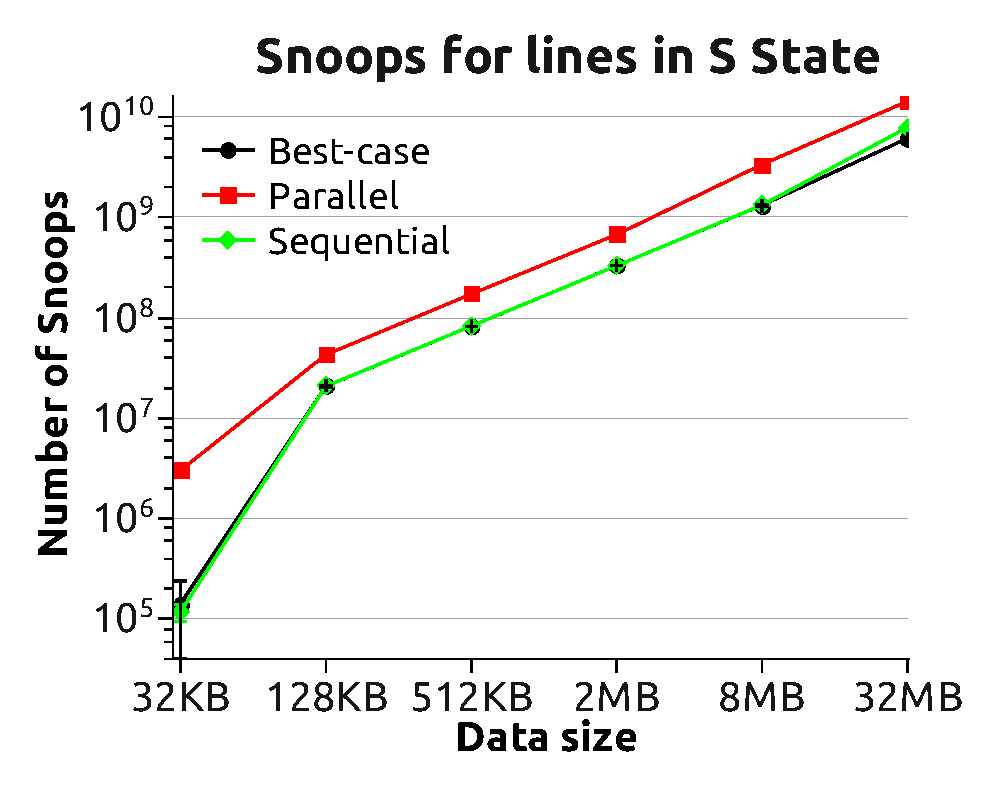
\includegraphics[width=.22\textwidth,height=3.25cm]{fig/HPC_snoop_share2}
	\label{fig:snoops_s}
	} 
\caption{Benchmark HPCs evaluation on Intel Q9550 processor: snoop requests for I and S states.}
\label{fig:snoop_req}
\end{figure}

Finally, the next experiment evaluates the number of snoop responses to bus transactions. Bus transactions are generated due to the cache coherence. For example, when a processor writes into a shared data (cache line in the S state), a bus transaction is generated to invalidate other data copies. The writing operation only ends when the snoop response for the bus transaction arrives. Figure~\ref{fig:HPC_ext_snoop_hitm2} shows the number of snoop responses to bus transactions that reach a cache line in the M state, that is, a core has written to a data and another core wants to read or write the same data.

\fig{HPC_ext_snoop_hitm2}{Benchmark HPCs evaluation on Intel Q9550 processor: external snoops HITM.}{width=.21\textwidth,height=3.25cm}

We can note that the curves in Figure~\ref{fig:HPC_ext_snoop_hitm2} are similar to the curves in Figure~\ref{fig:snoops_i}. This was expected because both threads have the same writing and reading operations. Figure~\ref{fig:snoops_i} has shown the number of times the L1 data cache of a core is snooped and Figure~\ref{fig:HPC_ext_snoop_hitm2} shows the number of snoop responses of this same core for a snoop request from the other core. Thus, both events are complementary and good options to monitor shared memory invalidations.
 
%Como usar o evento no escalonador: monitorar por um quantum, interrupcoes geradas quando o contador atinge um valor pre-definido
For instance, the scheduler could monitor the number of external snoops HITM and snoop requests for I state during a quantum in all cores. If the read value is greater than a threshold (5000 for example -- sequential and best-case applications have obtained up to 100 requests in a quantum of 10~ms) in two or more cores, the scheduler can detect memory invalidation activities in those threads running on different cores, and take a decision, as to schedule or not a thread or to stop it for a while in order to decrease the overhead associated to the memory coherency.

%Talvez uma meia culpa dizendo que a maioria dos processadores precisa de um suporte melhor de hardware para detectar isso de maneira mais facil.
\textbf{Improving the PMU support}. Initially, hardware designers have added PMU capabilities into processors to collect information for their own use~\cite{Tam:2007}. However, PMUs features have become useful for other performance measurements, such as energy management and scheduling decision. In consequence, the hardware designers are now adding more functionalities to PMUs, which can certainly help the software developer even more. Features like data address sampling, monitoring address space intervals, processing cycles spent in specific events, and interrupt generation when a pre-defined value is reached could be very useful for detecting memory coherency activities. We believe that the analysis made by this paper can help hardware designers to improve PMU features in multicore processors and their use in real-time applications.

% 
\section{Related Work}
\label{sec:related}
% 
% In the next subsections we summarize the main publications related to memory hierarchy in multicore systems and multicore scheduling that uses HPCs.
% 
% \subsection{Memory Hierarchy}
% 
Shared cache partitioning is the most common method used to address contention and provide real-time guarantees to multicore applications. Partitioning is used to isolate applications workloads that interfere each other and thus increasing predictability~\cite{Cho:2006b, Muralidhara:2010}. 
%Several hardware-~\cite{Suhendra2008} and software-based~\cite{Cho:2006b, Muralidhara:2010} %Zhang:2009, cache partitioning have been proposed in the last years. The software-based approach has the advantage to be completely transparent to applications and there is no need to special hardware support. 
% %The most common software-based technique is the \emph{page coloring}. This technique explores the translation from virtual to physical memory addresses presented in the virtual memory systems, in such a way that addresses from different applications are always mapped to pre-defined cache regions~\cite{Liedtke:1997, Cho:2006b}.
% Differently from the previous works, which focused on multi-application workloads, Chen analyzed different policies for managing shared caches for multi-threaded applications~\cite{YuChen:2009}. The work has shown that the shared-cache miss rate can be reduced by allocating a certain amount of space for shared data. Muralidhara proposed a dynamic software-based partitioning technique that partitions the shared cache space among threads of a given application~\cite{Muralidhara:2010}. At the end of each 15~ms interval, the technique uses HPCs information, such as cache hit/misses, cycle and instruction counts for each thread, in order to allocate different cache space based on individual thread performance. The objective is to speed up the critical path, that is, the thread that has the slowest performance and, consequently, improve the overall performance for the application. The results have shown a performance gain of up to 23\% over a statically partitioned cache~\cite{Muralidhara:2010}.  
% 
Another important research topic related to memory hierarchy in multicore architectures is the timing and delay analyses. A framework for estimating the worst-case response time of tasks sharing an instruction cache was developed by Suhendra et al.~\cite{Li2009}. However, this work assumes that data memory references (i.e., data cache) do not interfere in the tasks' execution time. We have shown in this paper that the data memory hierarchy poses an important influence in the application's execution time. %Moreover, the system model used by the authors is simple, it does not consider preemptions and data exchange among tasks are only done by message passing. 
\textit{Schedule-Sensitive} and \textit{Synthetic} are two methods to measure cache-related preemption and migration delays (CPMD)~\cite{Anderson2010a}. The evaluation shows that the CPMD in a system under load is only predictable for working set sizes that do not trash the L2 cache~\cite{Anderson2010a}. 
% 
% \subsection{Multicore Scheduling}
% 

Considering HPCs as an alternative to easily detect sharing pattern among threads and help scheduling decisions, Bellosa and Steckermeier were the first to suggest using HPCs to dynamically co-locate threads onto the same processor~\cite{Bellosa:1996}. Tam et al. use HPCs to monitor the addresses of cache lines that are invalidated due to cache-coherence activities~\cite{Tam:2007}. West et al.~\cite{West:2010} propose an online technique based on a statistical model to estimate per-thread cache occupancies online through the use of HPCs. However, data sharing is not considered by the authors.
%and to construct a summary data structure for each thread, which contains the addresses of each thread that are fetching from the cache. Based on the information from this data structure, the scheduler mounts a cluster composed of a set of threads, and allocates a cluster to a specific core. However, this approach is not feasible for UMA processors, since there is no performance gains in allocating a thread to a specific core. West et al.~\cite{West:2010} propose an online technique based on a statistical model to estimate per-thread cache occupancies online through the use of HPCs. However, data sharing is not considered by the authors.
% 
Another work to address shared resource contention via scheduling was proposed by Zhuravlev~\cite{Zhuravlev:2010}. The paper identifies the main problems that can cause contention in shared multicore processors (e.g., memory controller contention, memory bus contention, prefetching hardware, and cache space contention). The authors propose two scheduling algorithms (\textit{Distributed Intensity} - DI, and \textit{Distributed Intensity Online} - DIO). DI uses a threads' memory pattern classification as input, and distributes threads across caches such that the miss rates are distributed as evenly as possible. DIO uses the same idea, but it reads the cache misses online, through HPCs. %DIO performed better than the Linux CFS both in terms of average performance as well as execution time stability from different executions~\cite{Zhuravlev:2010}.
% 
Calandrino and Anderson have proposed a cache-aware scheduling algorithm~\cite{Calandrino:2009}. The algorithm uses HPCs to estimate the working set of each thread and to schedule them in order to avoid cache thrashing and provide real-time guarantees for soft real-time applications. However, to correctly estimate the working set, the threads must not share data and and the data size of the running threads must be less than the cache size. $FP_{CA}$ is a cache-aware scheduling algorithm that divides the shared cache space into partitions~\cite{Guan2009}. Tasks are scheduled in a way that at any time, any two running tasks' cache spaces (e.g., a set of partitions) are non-overlapped. A task can execute only if it gets an idle core and enough cache partitions.
% 
In general, all the above related work do not consider a multicore system where threads share data. We demonstrated through our benchmark evaluation that the contention for shared memory data can influence the application's execution time and lead to performance degradation and deadline losses. 

\section{Conclusion}
\label{sec:conc}

This paper evaluated the influence of contention for shared data memory in the context of real-time multicore applications. We have designed a benchmark in order to measure how the application's execution time is affected by the memory coherency hardware mechanism (e.g., snooping). The benchmark, composed of two versions of an application (sequential and parallel), was evaluated in 5 different processors with 3 different cache-coherence protocols (MESI, MOESI, and MESIF) and two memory architectures (UMA and ccNUMA). The results have shown that real-time applications mainly on top of UMA processors must consider the coherence between the memory hierarchy. A execution time degradation up to 3.87 times in the parallel version was obtained only because the contention for shared data memory. As a step forward to mitigate the problem, we analyze some hardware events that could be used by the OS scheduler at run-time to obtain a precise view of the data sharing activities between cores. As future work, we plan to integrate the studied HPCs into a real-time multicore scheduler.

%\section*{Acknowledgments}
%This work was partially supported by the Coordination for Improvement of Higher Level Personnel (CAPES) grant, project RH-TVD 006/2008, and by the German Research Council (DFG) under grant no. SCHR 603/7-1.

\bibliographystyle{unsrt}
\bibliography{references}

\end{document}
